\subsection{Unsynchronized Transmitter and Receiver}

\begin{figure*}[!t]
   \centering
   \begin{subfigure}[h]{0.25\textwidth}
      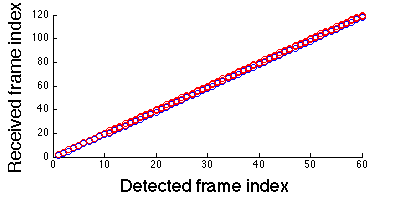
\includegraphics[width=\textwidth]{fig/tx_15_new.png}
      \caption{tx = 15 fps} \label{fig:tx_15fps}
   \end{subfigure}%
   ~
   \begin{subfigure}[h]{0.25\textwidth}
      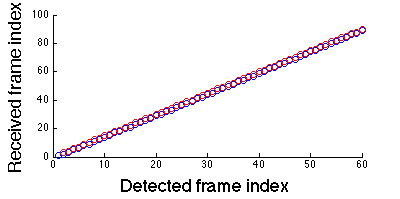
\includegraphics[width=\textwidth]{fig/tx_20_new.png}
      \caption{tx = 20 fps} \label{fig:tx_20fps}
   \end{subfigure}%
   ~  
   \begin{subfigure}[h]{0.25\textwidth}
      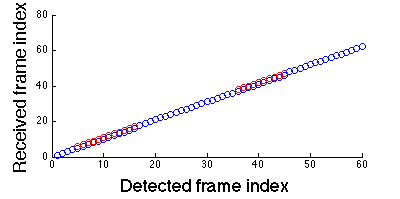
\includegraphics[width=\textwidth]{fig/tx_29_new.png}
      \caption{tx = 29 fps} \label{fig:tx_29fps}
   \end{subfigure}%
   ~
   \begin{subfigure}[h]{0.25\textwidth}
      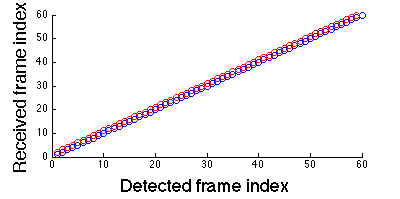
\includegraphics[width=\textwidth]{fig/tx_30_2_new.png}
      \caption{tx = 30 fps} \label{fig:tx_30fps_2}
   \end{subfigure}%
   \\
   \begin{subfigure}[h]{0.25\textwidth}
      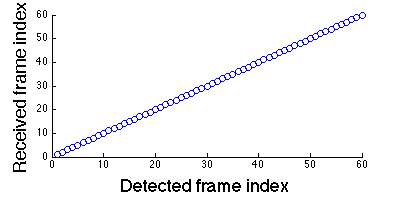
\includegraphics[width=\textwidth]{fig/tx_30.png}
      \caption{tx = 30 fps} \label{fig:tx_30fps}
   \end{subfigure}%
   ~   
   \begin{subfigure}[h]{0.25\textwidth}
      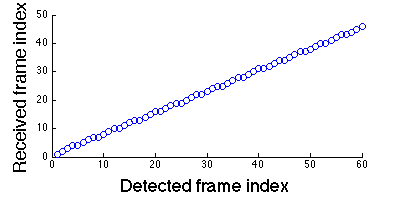
\includegraphics[width=\textwidth]{fig/tx_40.png}
      \caption{tx = 40 fps} \label{fig:tx_40fps}
   \end{subfigure}%
   ~
   \begin{subfigure}[h]{0.25\textwidth}
      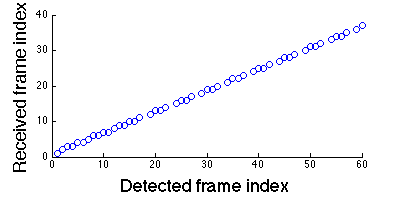
\includegraphics[width=\textwidth]{fig/tx_50.png}
      \caption{tx = 50 fps} \label{fig:tx_50fps}
   \end{subfigure}%
   ~
   \begin{subfigure}[h]{0.25\textwidth}
      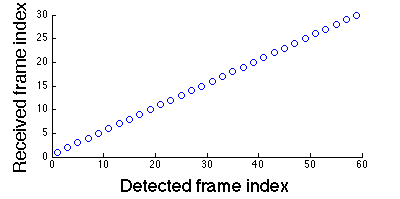
\includegraphics[width=\textwidth]{fig/tx_60.png}
      \caption{tx = 60 fps} \label{fig:tx_60fps}
   \end{subfigure}%
   \caption{Received frame patterns under different tx fps}
   \label{fig:diff_tx}
\end{figure*}

\subsubsection{The Problem}

As the transmitting light and the receiving camera are not synchronized, the transmitting frame rate and the receiving frame rate are usually not the same. 
As mentioned is~\cite{hu2013lightsync}, the received frame rate exhibits more variability for several reasons. It described as follows: HTC One X camera appears to record videos are 24 fps, but the camera callback API can only support saving the frames at 15 to 20 fps. The callback slows down when there is insufficient memory available in the system. The frame rate on the Samsung Galaxy S III is only stable if the CPU is locked to its maximum frequency with its setCPU app. Otherwise, it fluctuates hugely between 21 to 29 fps for an entirely white foreground, and have an average of around 25 fps. Even when the frame rate appears steady, the inter-frame interval still varies. 

% In our design, we assume that the ratio $fps_{tx}$ / $fps_{rx}$ is not more than 2 or less than 0.9, which means the receive frame rate is between 15 and 33 fps when the transmitting frame rate is 30 fps. Note that this can be changed with straightforward modifications to our design to allow a larger variability of frame rate. 

\textbf{Received frame patterns.} We follow the experiement in~\cite{hu2013lightsync}, given various potential combinations of the transmitting and receiving frame rates, we perform a simple experiment to study the received frame pattern. We transmit the data at several frame rates, and record the video with the PointGrey Flea3 camera~\cite{pointgrey_flea} with 30 fps. 

\autoref{fig:diff_tx} shows the received frame pattern. For each received frame, we can detect which of the originally transmitted frames corresponds to it, and plot a circle for each detected frame. When two or more detected frame indices correspond to the same received frame index, this captured frame contains a \textbf{mixture of two or more transmitted symbols}. When two or more received frame indices correspond to the same detected frame index, these captured frames have \textbf{redundant transmitted symbols}. Any gap between consecutive received frame indices indicates a \textbf{symbol loss}. 

At 15 fps and 20 fps, we capture at least one complete frame with a full symbol. However, other frames show that the mixed frames and redundant frames are also possible due to random phase offsets. When the transmitting rate is close to the receiving rate - 30 fps, mixed frames would be received for a few consecutive frames. Even when the transmitting frame rate is exactly 30 fps, mixed frames can still occur, in which case, it would always be the case received due to the constant phase offset, as shown in \autoref{fig:tx_30fps_2}. In the other case, a single transmitted symbol would always be received in each frame, as shown in \autoref{fig:tx_30fps}.
As the transmitting rate increases further, we start to experience mixed and missed symbols at times.

% Since the camera records the videos at 30 fps, detecting the same number of transmitted frames requires receiving far more frames at a low transmitting rate. Therefore, the scales of the vertical axis are different across the subfigures of \autoref{fig:diff_tx}.

\subsubsection{The Probability}
\label{sec:unsync}
To figure out the symbol loss and mixed frame problems, we first want to know how often do they happen, thus we derive the probabilities under different conditions. In addition, we want to know what factors affect them and how to address them. 

\textbf{Case I: When the transmitting frame rate is higher than the receiving frame rate,}
there could be symbol loss, defined as no part of the transmitting frame duration of a particular symbol is covered by the exposure time of any receiving image frame. 
\autoref{fig:miss} illustrates the missing symbols. 
Let the transmitting frame duration be $T_{f,tx}$ (symbol time), the receiving frame duration be $T_{f,rx}$, and the Y size of the image area illuminated by the transmitting light be $H$. The gray part is the time gap that the camera is not receiving the transmitting symbols. If $T_{f,tx} < T_{f,rx} - H T_r$, which means the transmitting symbols may appear in the gray part, then a symbol loss is possible. In that case, the probability of a symbol lost is given by
\begin{equation}
	P_{\operatorname{miss}}=\frac{T_{f,rx} - H T_r - T_{f,tx} }{T_{f,rx}} \qquad \textrm{.}
\end{equation}

We can see that the probability of the symbol loss in \autoref{fig:miss} is around 1/2, which means there is a symbol loss followed by every received symbol. 


A more common event which could happen when the transmitting frame duration and the receiving frame duration are different is that in a single image frame there could be multiple image areas each corresponding to a symbol. In other words, a mix of different symbols in a single receiving image frame. 
\autoref{fig:mix} illustrates the mixed frames. If the boundary between two consecutive transmitting symbols locates in the red part, during which the camera is receiving the transmitting symbols, then there is a mixed frame.
The probability for this event is given by
\begin{equation}
P_{\operatorname{mix}}=\begin{cases} \frac{H T_r}{T_{f,tx}}, & \textrm{if\;} T_{f,tx} \geq H T_r \\
1, & \textrm{otherwise.} \end{cases}
\end{equation}

We can see that the probability of the mixed frame in \autoref{fig:mix} is around 1/3. 

\begin{figure}[!t]
  \centering
  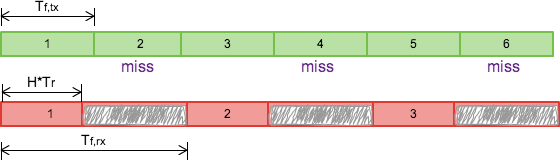
\includegraphics[scale=0.35]{fig/miss.png}
  \caption{Missing symbol illustration.}
  \label{fig:miss}
\end{figure}

\begin{figure}[!t]
  \centering
  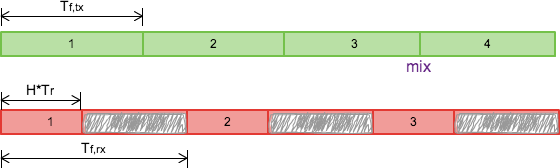
\includegraphics[scale=0.35]{fig/mix.png}
  \caption{Mixed frame illustration.}
  \label{fig:mix}
\end{figure}

A mixed frame is a very common and periodic event. Even when the transmitting and the receiving frame durations are very close to each other, mixed frames would be received for a few consecutive frames. After receiving a few frames with only a single symbol, consecutive mixed frame would appear again. \autoref{fig:mix_photo} shows the received frame with mixed symbols.
If the boundary of the image areas corresponding to different symbols is not determined, then the period detection algorithm would output one value. The value would usually be closer to the signal period of the symbol that occupies a larger image area, but usually has a large error.  

% \begin{figure}[!t]
%   \centering
%   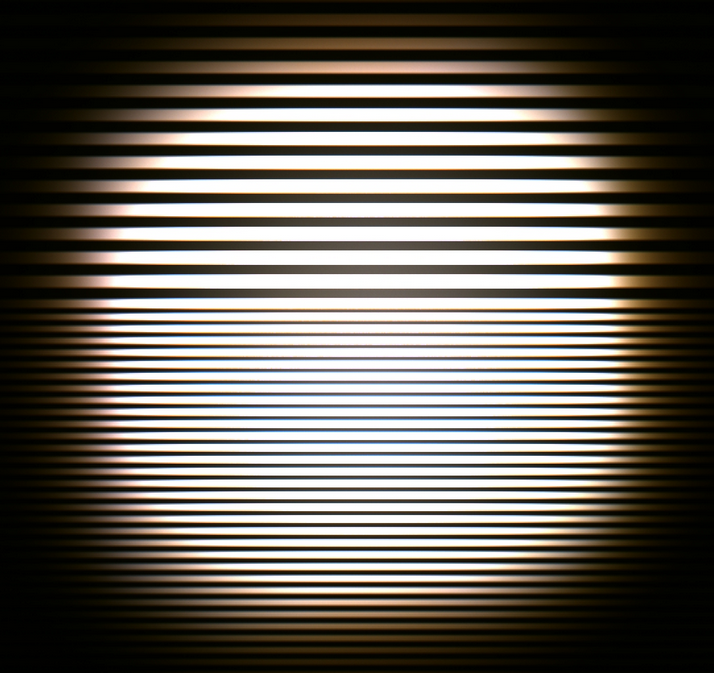
\includegraphics[scale=0.1]{fig/mix_photo.png}
%   \caption{Received frame with mixed symbols.}
%   \label{fig:mix_photo}
% \end{figure}

\textbf{Case II: When the transmitting frame rate is lower than the receiving frame rate,}
a redundant symbol is possible. Although no information is lost, the receiver still needs to detect a redundant symbol so that it can be dropped to obtained the correct symbol sequence.  


On the other hand, a mixed frame is also possible in this case. The probability for a mixed frame is given by
\begin{equation}
P_{\operatorname{mix}}=\frac{H T_r}{T_{f,tx}} \qquad \textrm{.}
\end{equation}
which is same as the probability in Case I.
We can see that the probability of the mixed frame in \autoref{fig:mix2} is around 1/3. 

According to the probability of lost symbol and mixed frame, the transmitting frame duration ($T_{f,tx}$), the receiving frame duration ($T_{f,rx}$), the height of the LED in the image ($H$), and the read-out time of camera sensor ($T_r$) and the factors which may affect the probabilities. We will introduce and evaluate how well our design address these issues in the following chapters.
